% =============================================================================
%  CSE 200 -- LaTeX Online 1 : COMPLETE ANNOTATED DEMO
% =============================================================================
%
%  WHAT THIS IS
%  ------------
%  One compilable document containing every LaTeX construct that has appeared
%  in the nine past papers in prev_onlines/, each one preceded by a comment
%  block saying what it does, why it is written that way, and what usually
%  goes wrong.  Read the source on one side, the PDF on the other.
%
%  WHERE TO PUT IT
%  ---------------
%  This file must sit in the CSE200/ folder (next to prev_onlines/), because
%  the figure examples load the real images from:
%      prev_onlines/22_A2/A.PNG  B.PNG  C.PNG
%      prev_onlines/23_A1/trefoil_knot.png
%      prev_onlines/23_B1/rc_circuit.png
%      prev_onlines/23_C2/sun.png mercury.png venus.png earth.png mars.png
%                          jupiter.png saturn.png uranus.png neptune.png
%
%  HOW TO COMPILE
%  --------------
%      latexmk -pdf cse200-demo.tex          <-- easiest, does every pass
%
%  or by hand (the bibliography needs all four passes):
%      pdflatex cse200-demo        % pass 1: writes .aux with every \label and \cite
%      bibtex   cse200-demo        % builds .bbl from refs.bib  (NO extension!)
%      pdflatex cse200-demo        % pass 2: pulls in the .bbl
%      pdflatex cse200-demo        % pass 3: fixes the [1] numbers and the ToC
%
%  If you skip passes you get  ??  for references and  [?]  for citations.
%  It needs refs.bib in the same folder (shipped alongside this file).
%
%  CONTENTS
%  --------
%   1 Text formatting          8 Figures
%   2 Colour                   9 Code listings
%   3 Lists                   10 Algorithms and pseudocode
%   4 Spacing and breaks      11 Cross-references, footnotes, hyperlinks
%   5 Mathematics             12 Citations and bibliography
%   6 Theorems and proofs     13 TikZ
%   7 Tables                  14 Two-column layout
%
%  Beamer lives in the companion file cse200-demo-beamer.tex, because beamer
%  is a document *class* -- it cannot share a file with an article.
% =============================================================================


% =============================================================================
%  THE DOCUMENT CLASS
% =============================================================================
%  article   = what every past paper uses.
%  11pt      = base font size (default is 10pt).
%  a4paper   = A4 instead of US letter.
%  Add  twocolumn  here if the model paper is two-column (23_A1, 23_C1):
%      \documentclass[11pt,a4paper,twocolumn]{article}
\documentclass[11pt,a4paper]{article}


% =============================================================================
%  THE PREAMBLE  --  everything between \documentclass and \begin{document}
% =============================================================================
%  Nothing printable goes here. This list is a superset of every package used
%  across prev_onlines/ and sir_template.tex. Typing it takes ninety seconds
%  and immunises you against "Undefined control sequence" for the whole exam.

\usepackage[T1]{fontenc}      % lets a straight " render inside a code listing
\usepackage[margin=1in]{geometry}   % page margins; also top=/bottom=/left=/right=
\usepackage{graphicx}         % \includegraphics
\usepackage{float}            % the [H] "put it exactly here" float option
\usepackage{wrapfig}          % wrapfigure -- text flows around an image
\usepackage{caption}
\usepackage{subcaption}       % the subfigure environment
\usepackage{booktabs}         % \toprule \midrule \bottomrule
\usepackage{array}            % p{} m{} b{} paragraph columns, >{} column prefixes
\usepackage{multirow}         % \multirow
\usepackage{enumitem}         % list label / spacing control
\usepackage[table]{xcolor}    % \textcolor AND \rowcolor \cellcolor
                              % ^^^^^^^ the [table] option is what enables
                              %         coloured rows and cells. Forget it and
                              %         \rowcolor silently does nothing.
\usepackage{amsmath, amssymb, amsfonts}   % all the maths
\usepackage{amsthm}           % \newtheorem and the proof environment
\usepackage{listings}         % code listings, compiles with plain pdflatex
\usepackage{algorithm}        % the "Algorithm 1" float
\usepackage{algpseudocode}    % the pseudocode body (\State \If \While ...)
\usepackage{comment}          % \begin{comment} ... \end{comment}
\usepackage{tikz}             % drawings
\usetikzlibrary{positioning}  % right=of / above=of
\usetikzlibrary{calc}         % ($(a)!0.5!(b)$) arithmetic on coordinates
\usetikzlibrary{fit}          % a node fitted around other nodes
\usetikzlibrary{arrows}       % the primed arrow tips: stealth' latex' to'
\usepackage[numbers]{natbib}  % \citep \citet, numeric [1] style
\usepackage{refcount}         % \getrefnumber, used to re-use a footnote number
\usepackage{hyperref}         % \href \url, clickable cross-references
% GOTCHA: hyperref must be loaded LAST (or nearly last). It redefines a lot of
% internals, and packages loaded after it can silently break its references.

% Link colours. Without colorlinks=true you get ugly coloured boxes instead.
\hypersetup{
    colorlinks=true,
    urlcolor=blue,      % \href and \url
    citecolor=black,    % \cite
    linkcolor=black     % \ref and table-of-contents entries
}

% -----------------------------------------------------------------------------
%  COLOUR DEFINITIONS
% -----------------------------------------------------------------------------
%  RGB (capitals) takes integers 0-255.  rgb (lowercase) takes fractions 0-1.
%  HTML takes a hex string.  gray takes a single 0-1 value.
\definecolor{customblue}{RGB}{0, 76, 153}
\definecolor{softgreen}{RGB}{226, 245, 236}
\definecolor{softred}{RGB}{255, 232, 232}
\definecolor{softyellow}{RGB}{255, 247, 214}
\definecolor{lightgray}{gray}{0.9}
\definecolor{myorange}{HTML}{E2A75C}

% -----------------------------------------------------------------------------
%  LISTINGS STYLE  (the course-taught style, from sir_template.tex)
% -----------------------------------------------------------------------------
%  Set once here; every \begin{lstlisting} in the document inherits it.
\lstset{
    basicstyle=\ttfamily\small,
    keywordstyle=\color{customblue}\bfseries,
    commentstyle=\color{teal!70!black},
    stringstyle=\color{red!70!black},
    frame=single,                       % box around the listing
    numbers=left,                       % line numbers in the left margin
    numberstyle=\tiny\color{gray},
    breaklines=true,                    % wrap long lines instead of overflowing
    showstringspaces=false,
    columns=fullflexible,
    tabsize=4
}

% -----------------------------------------------------------------------------
%  MATH OPERATOR AND THEOREM DECLARATIONS
% -----------------------------------------------------------------------------
%  The star in \DeclareMathOperator* puts limits BELOW the operator, like \sum.
\DeclareMathOperator*{\argmax}{arg\,max}

%  \newtheorem{env}{Printed name}            -> numbered 1, 2, 3 ...
%  \newtheorem{env}{Printed name}[section]   -> numbered 3.1, 3.2 ...
%  \newtheorem{env}[other]{Printed name}     -> shares "other"'s counter
\newtheorem{proposition}{Proposition}
\newtheorem{theorem}{Theorem}[section]
\newtheorem{lemma}[theorem]{Lemma}          % lemmas and theorems share a counter
\theoremstyle{definition}                   % upright body instead of italic
\newtheorem{definition}{Definition}

% -----------------------------------------------------------------------------
%  TIKZ STYLES  (define once, reuse by name)
% -----------------------------------------------------------------------------
\tikzset{
    block/.style={draw, rounded corners, minimum width=2.4cm,
                  minimum height=0.9cm, align=center, fill=blue!10},
    neuron/.style={circle, draw, minimum size=7mm},
    arrowline/.style={->, thick, red}
}

% -----------------------------------------------------------------------------
%  TITLE BLOCK
% -----------------------------------------------------------------------------
%  Three patterns show up in the past papers. Pattern 2 is used below; the
%  other two are kept as comments so you can swap them in.
%
%  Pattern 1 -- plain, one author:
%      \title{Mathematical Foundations of Image Synthesis}
%      \author{Your Name (Your Student ID)}
%      \date{\today}          % \date{} prints no date at all
%
%  Pattern 3 -- the authblk package (needs \usepackage{authblk}):
%      \title{\textsc{The Solar System}}       % \textsc = small caps title
%      \author[1]{Johannes Kepler}
%      \affil[1]{Imperial Mathematician, Prague}
%
%  Pattern 2 -- superscript affiliations, hand-built, no package needed.
%  This is what 23_B1, 23_A2, 23_B2 and the makeup paper use.
%  \\[6pt] is a line break plus 6pt of extra vertical space.
\title{CSE 200 Annotated LaTeX Demo \\[4pt]
       \large Every construct from \texttt{prev\_onlines/}, with commentary}
\author{
Zarif Ishmam$^{1}$, Pierre-Simon Laplace$^{2}$, and Johannes Kepler$^{3}$\\[6pt]
\small $^{1}$Department of CSE, BUET, Dhaka, Bangladesh\\
\small $^{2}$Acad\'emie des Sciences, Paris, France\\
\small $^{3}$Imperial Mathematician, Prague
}
\date{\today}


% =============================================================================
\begin{document}
% =============================================================================

\maketitle

% \tableofcontents builds itself from the .toc file written during the PREVIOUS
% compile, so it is empty on run 1 and correct on run 2. Both 23_C1 and 23_C2
% follow it with \newpage to keep it on a page of its own.
\tableofcontents
\newpage


% #############################################################################
\section{Text formatting}
% #############################################################################
% Everything in this section is built into LaTeX -- no package required.

% --- the font-shape commands -------------------------------------------------
% Each takes an argument. There are also switch forms ({\bfseries ...}) that
% stay in effect until the enclosing group ends.
This sentence has \textbf{bold text}, \textit{italic text},
\emph{emphasized text}, and \underline{underlined text}.
\textsc{Small Caps}, \texttt{typewriter}, \textsf{sans serif},
\textrm{roman} and \textsl{slanted} also turn up.

% GOTCHA: \textit vs \emph.  \textit ALWAYS italicises.  \emph is semantic:
% it italicises inside upright text but flips back to upright inside italic
% text. Prefer \emph for emphasis.  Compare:
\textit{outer italic \textit{inner stays italic} back}\ vs.\
\textit{outer italic \emph{inner flips upright} back}

% --- the ten font sizes ------------------------------------------------------
% These are SWITCHES, not commands with arguments, so they are wrapped in
% braces to limit how far they reach.
Font sizes: {\tiny tiny} {\scriptsize scriptsize} {\footnotesize footnotesize}
{\small small} {\normalsize normalsize} {\large large} {\Large Large}\\
{\LARGE LARGE} {\huge huge} {\Huge Huge}.

% --- quotes, dashes, escapes -------------------------------------------------
% GOTCHA: typing "quoted" gives you two RIGHT-hand quotes at both ends.
% The correct input is two backticks then two apostrophes.
Quotes: ``proper double quotes'' and `single quotes'.
Dashes: inter-word hyphen, a number range 1--9 (en dash),
and an em dash---like this---for an aside.

% The ten characters that must be escaped with a backslash:
Escapes: 100\% \& \$ \# \_ \{ \} and \textbackslash{} \~{} \^{}.

\bigskip
% \verb prints its argument exactly as typed. It takes ANY delimiter character
% that does not appear inside the text itself: \verb|...| \verb+...+ \verb!...!
Inline verbatim: \verb|\textbf{this is not bolded}| and \verb+100% raw+.


% #############################################################################
\section{Colour}
% #############################################################################
% Needs \usepackage[table]{xcolor}. Every 2023 paper has marks for "Colors".

% --- \textcolor wraps a run of text ------------------------------------------
\textcolor{red}{Colored text in red} and
\textcolor{customblue}{a phrase in the custom blue defined in the preamble}.

% --- \color is a SWITCH: it stays on until the enclosing group ends -----------
{\color{red} Everything inside these braces is red.} Back to black.

% --- highlighting and boxing -------------------------------------------------
A \colorbox{softyellow}{short highlighted note} and a
\fcolorbox{red}{softyellow}{boxed and filled} phrase.

% --- colour mixing -----------------------------------------------------------
% A!p      = p percent of A mixed with white
% A!p!B    = p percent of A mixed with (100-p) percent of B
\textcolor{blue!40}{40\% blue on white}, and
\textcolor{teal!70!black}{teal darkened with 30\% black}.

\medskip
% This two-colour contrast pattern is exactly what 23_B1 and 23_C2 ask for:
% two \textcolor runs inside one sentence.
\textcolor{blue}{In the time domain a system is described by a differential
equation}, whereas \textcolor{red}{in the Laplace domain the same system is
described by a rational algebraic expression}.

The 19 predefined names are: red, green, blue, cyan, magenta, yellow, black,
gray, white, darkgray, lightgray, brown, lime, olive, orange, pink, purple,
teal and violet.


% #############################################################################
\section{Lists}
% #############################################################################
% Three environments, nestable four deep. \usepackage{enumitem} adds the
% label= and spacing keys used below.

\subsection{Nested and mixed lists}

% The starred counter commands inside label= expand to the item number:
%   \arabic*  1 2 3      \alph*  a b c      \Alph*  A B C
%   \roman*   i ii iii   \Roman* I II III
% \item[X] overrides the label for ONE item only.
\begin{enumerate}[label=\arabic*.]
    \item System Setup
    \begin{itemize}
        \item Install software packages
        \item Configure hardware
        \item[!] Verify connections      % one-off label override
    \end{itemize}

    \item Simulation Steps
    \begin{enumerate}[label=(\alph*)]
        \item Initialize parameters
        \item Run simulation
        \begin{itemize}[label=-]         % label for the WHOLE list
            \item Monitor CPU usage
            \item[$\rightarrow$] Record intermediate results
        \end{itemize}
        \item Analyze outputs
    \end{enumerate}
\end{enumerate}

\subsection{Every label format the past papers use}

\begin{enumerate}[label={(\Roman*)}]      % 23_C2, 23_B2
    \item Roman-numbered item
    \item Another roman-numbered item
\end{enumerate}

\begin{enumerate}[label=(\Alph*)]          % 23_C1 zero classification
    \item Capital-lettered item
\end{enumerate}

\begin{enumerate}[label=(\roman*)]         % 23_C1 companion points
    \item Lowercase roman item
    \item Another one
\end{enumerate}

% GOTCHA: label={I} is LITERAL TEXT, not a counter. Every item prints "I".
% 23_C2's source really does contain this quirk -- reproduce it if you see it.
\begin{enumerate}[label={I}]
    \item Both of these items print the same label
    \item ...because {I} is literal, not \textbackslash Roman*
\end{enumerate}

% label= (empty) removes the marker entirely, which lets \textbf act as a
% run-in heading. This is the 23_B1 "Differential equations / Electrical
% circuits" pattern.
\begin{enumerate}[leftmargin=*, label=]
    \item \textbf{Differential equations} $\oplus$ initial conditions are
          included automatically; \\
          $\oplus$ derivatives become algebraic expressions.
    \item \textbf{Control and signal systems} $\oplus$ stability is studied
          through poles; \\
          $\oplus$ common test inputs include:
        \begin{itemize}
            \item[$\rhd$] the unit-step input;
            \item[$\rhd$] the impulse input;
            \item[$\rhd$] sinusoidal inputs.
        \end{itemize}
\end{enumerate}

\subsection{Symbol bullets}
% Any maths symbol works as a label. If a marker in the model paper looks
% bizarre it is almost certainly \item[$\somesymbol$] -- search a symbol list
% or use detexify rather than trying to draw it.
\begin{itemize}
    \item[$\dagger$]     \verb|$\dagger$|     -- used by 23\_C2
    \item[$\diamond$]    \verb|$\diamond$|    -- 23\_C2, 23\_A2, makeup
    \item[$\oplus$]      \verb|$\oplus$|      -- 23\_B1, 23\_A1
    \item[$\rhd$]        \verb|$\rhd$|        -- 23\_B1
    \item[$\nmid$]       \verb|$\nmid$|       -- 23\_C1
    \item[$\ni$]         \verb|$\ni$|         -- 23\_C1
    \item[$\ast$]        \verb|$\ast$|
    \item[$\star$]       \verb|$\star$|
    \item[$\circ$]       \verb|$\circ$|
    \item[$\bullet$]     \verb|$\bullet$|
    \item[$\rightarrow$] \verb|$\rightarrow$|
    \item[\#]            \verb|\#| -- a plain escaped character works too
\end{itemize}

\subsection{Description lists and spacing control}

% description = bold run-in terms. This is the "Arc / Crossing / Orientation"
% block in 23_A1 and the API/LAN/ASCII list in the beamer tutorial.
\begin{description}
    \item[Arc] A continuous segment between two undercrossings.
    \item[Crossing] A point where one projected strand passes over another.
    \item[Orientation] A selected direction of travel around the knot.
\end{description}

% enumitem spacing keys: leftmargin, itemsep, topsep, parsep, noitemsep
\begin{itemize}[leftmargin=*, itemsep=0.6em, topsep=0pt]
    \item Widely spaced item, flush to the left margin
    \item Another one
\end{itemize}

\begin{itemize}[noitemsep, topsep=0pt]
    \item Tight item
    \item Another tight item
\end{itemize}


% #############################################################################
\section{Spacing, breaks and alignment}
% #############################################################################

% --- horizontal space --------------------------------------------------------
Horizontal: a\hspace{1cm}b, a\quad b, a\qquad b, a$\,$b (thin), a\ b (forced).
\hspace{20px} is also legal -- 23\_B1 uses it inside equations.

% \hfill pushes what follows to the right-hand margin:
Left side \hfill Right side

\medskip
% --- vertical space ----------------------------------------------------------
% \smallskip \medskip \bigskip are the three named vertical gaps.
% \vspace{...} takes any length. \par\medskip ends the paragraph first --
% that is the idiom used between rows of subfigures.
This paragraph is followed by \verb|\vspace{0.8cm}|.
\vspace{0.8cm}

And this one comes after it.

% --- breaks ------------------------------------------------------------------
% \\           line break inside the same paragraph (no indent on the next line)
% blank line   new paragraph (indented)
% \newline     same as \\ but only valid in ordinary paragraph text
% \newpage     break to a new page
% \clearpage   break AND flush every pending float
% \noindent    kill the first-line indent of this paragraph only
A line break\\comes before this text, so there is no indent.

\noindent This paragraph starts with \verb|\noindent| so it is flush left.

% --- alignment ---------------------------------------------------------------
% GOTCHA: \begin{center} adds vertical space above and below; \centering does
% not. Inside a figure or table float, always use \centering.
\begin{center}
    This block is centred by the \texttt{center} environment.
\end{center}
\begin{flushleft}
    This block is ragged right.
\end{flushleft}
\begin{flushright}
    This block is ragged left.
\end{flushright}


% #############################################################################
\section{Mathematics}
% #############################################################################
% Worth about 31\% of the marks. Everything here needs
% \usepackage{amsmath, amssymb, amsfonts}.

\subsection{Inline versus display}

% Inline maths squashes big operators to keep the line height sane.
Inline maths: $x^2 + 1$, or with the newer delimiters \(x^2 + 1\).

% Display maths, unnumbered. $$...$$ is the old TeX form and appears all over
% prev_onlines/; \[...\] is the modern form and gives better error messages.
$$ f(t) \xrightarrow{\mathcal{L}} F(s) $$
\[ V_{\mathrm{in}}(s) = \frac{V_0}{s} \]

% Display maths, numbered. equation is the ONLY one of these that produces a
% number you can \ref to.
\begin{equation}
    L = I_{ij} \cdot \cos(\theta) + R^2
    \label{eq:sample}
\end{equation}

% The starred form suppresses the number.
\begin{equation*}
    c^2 = a^2 - b^2
\end{equation*}

\subsection{Scripts, Greek letters and named operators}

% GOTCHA: only ONE token is lifted by ^ or _. Always brace anything longer.
%   $x^10$  prints x to the power 1, followed by a 0
%   $x^{10}$ is what you meant
Superscripts and subscripts: $x^2$, $x_i$, $x_i^2$, $x_{i_2}$, $e^{x^2}$,
$T_M^2$, $\theta_i(t)$, $n^+(D)$, $t^{-1}$ and $x^{10}$.

Lowercase Greek: $\alpha \beta \gamma \delta \epsilon \varepsilon \zeta \eta
\theta \vartheta \iota \kappa \lambda \mu \nu \xi \pi \rho \sigma \tau
\upsilon \phi \varphi \chi \psi \omega$.

Uppercase Greek: $\Gamma \Delta \Theta \Lambda \Xi \Pi \Sigma \Upsilon \Phi
\Psi \Omega$. (The ones that look like Latin letters -- A, B, E -- have no
command; just type them.)

% GOTCHA: a bare  sin  inside maths is read as the product of three variables
% and comes out italic with wrong spacing. Always use the \sin form.
Named operators: $\sin\theta$, $\cos$, $\tan$, $\log$, $\ln$, $\exp$, $\min$,
$\max$, $\gcd$, $\deg$, $\dim$, $\det(K)$, $\arg$.

Your own operator, with limits underneath: $\argmax_{x} f(x)$.

\subsection{Fractions, roots and sized delimiters}

% \frac shrinks when inline; \dfrac is always display-size; \tfrac always small.
% A table cell is text-size, which is why 23_B1's Laplace table uses \dfrac
% everywhere together with \renewcommand{\arraystretch}{1.8}.
Fractions: $\frac{a}{b}$ (frac), $\dfrac{a}{b}$ (dfrac), $\tfrac{a}{b}$ (tfrac),
$\frac{n!}{s^{n+1}}$, $\frac{1}{2}\sqrt{3}$.

Roots: $\sqrt{2x+1}$, $\sqrt[3]{x}$, $\sqrt[5]{2x+1}$.

% \left and \right auto-size to their contents and MUST be paired.
% \left. or \right. makes one side invisible -- that is how you write an
% evaluation bar.
Sized delimiters:
$\left( \dfrac{1}{x^2+1} \right)$,
$\left[ \cdot \right]$,
$\left\{ \cdot \right\}$,
$\left| \cdot \right|$,
$\left\| v \right\|$,
$\left\lceil \log_4 M \right\rceil$ (ceiling, 23\_B2),
$\left\lfloor (\mathit{low}+\mathit{high})/2 \right\rfloor$ (floor),
and one-sided: $\left. \dfrac{dy}{dx} \right|_{x=1}$.

Fixed sizes when you do not want the automatic choice:
$\big( \Big( \bigg( \Bigg($.

\subsection{Sums, products, integrals and limits}

% In display mode the limits sit above and below; inline they sit beside.
% \limits and \nolimits force one or the other; \displaystyle forces the
% full display size mid-paragraph.
\[ \sum_{i=1}^{n} x_i \qquad \prod_{p \text{ prime}} \left(1 - p^{-s}\right)^{-1} \]
\[ \int_{0}^{\infty} e^{-st} f(t)\,dt \qquad \int_{2}^{x} \frac{dt}{\log t} \]

% \, is a thin space. The convention is to put one before the d of an integral.
Other big operators: $\iint$, $\oint$, $\bigcup_{i}$, $\bigcap_{i}$.

Limits: $\lim_{x \to a} f(x)$ inline squashes, whereas
$\lim\limits_{x \to a} f(x)$ forces the limit underneath, and
$\displaystyle\sum_{i=1}^{n} x_i$ forces the full display size.

\subsection{Multi-line derivations: the four environments}

% This single distinction is worth several marks in every 2023 paper.
% Ask one question of the model article: HOW MANY EQUATION NUMBERS does the
% block have?
%
%   align                 -> one number PER LINE
%   equation + split      -> ONE number for the whole block
%   align* / equation*    -> NO number
%   gather                -> one per line, but no alignment point
%
% & marks the alignment column (put it just before the =);  \\ ends a line.

% (a) align -- each line numbered. This is the 23_makeup style.
\begin{align}
    \frac{x}{100} + 45 &= 45 + \frac{4000 - x}{100} \\
    2x &= 4000, \quad x = 2000
\end{align}

% (b) equation + split -- one number for the whole derivation. 23_B1 style.
\begin{equation}
\begin{split}
    \mathcal{L}\{1\} &= \int_{0}^{\infty} e^{-st}\,dt \\
                     &= \left[-\frac{1}{s}e^{-st}\right]_{0}^{\infty} \\
                     &= \frac{1}{s}.
\end{split}
\label{eq:laplace-one}
\end{equation}

% (c) equation* + split -- no number at all. 23_C2 style.
\begin{equation*}
\begin{split}
    \frac{T_M^2}{T_E^2} &= \frac{a_M^3}{a_E^3} \\
    T_M &= T_E \left( \frac{a_M}{a_E} \right)^{3/2}
         \approx (1.524)^{3/2} \approx 1.88 \text{ years}.
\end{split}
\end{equation*}

% (d) align + split -- implication arrows down the left margin. The \implies
% goes BEFORE the &, so it hangs off the left of the alignment point.
\begin{align}
    \begin{split}
    RC \left[ sV_{C}(s) - v_{C}(0) \right] + V_{C}(s) &= V_{in}(s), \\
    \implies RCsV_{C}(s) + V_{C}(s) &= V_{in}(s), \\
    \implies V_{C}(s)(RCs + 1) &= V_{in}(s).
    \end{split}
    \label{eq:laplace-process}
\end{align}

% (e) gather -- centred lines, each numbered, with NO alignment point.
\begin{gather}
    a = b + c \\
    d = e
\end{gather}

% NOTE: split must live inside equation. "aligned" is the free-standing version
% you can drop anywhere, including inside another formula.

\subsection{Piecewise functions}

% GOTCHA: never type a bare word inside maths -- "if" becomes the product of
% the variables i and f, italic and badly spaced. Wrap it in \text{...}, and
% note the trailing space INSIDE the braces: \text{if }
\[
|y| = \begin{cases}
    y  & \text{if } y \geq 0 \\
    -y & \text{if } y < 0
\end{cases}
\]

\[
p(t) = \begin{cases}
    0,          & t < 0, \\
    e^{-t},     & 0 \le t < 3, \\
    \ln(t - 2), & t \ge 3
\end{cases}
\]

% A numbered piecewise block -- the label goes on the equation, not the cases.
\begin{equation}
\sigma(K) = \begin{cases}
    0,  & \text{if } K \text{ is the unknot,} \\
    -2, & \text{if } K \text{ is the right-handed trefoil,} \\
    2,  & \text{if } K \text{ is the left-handed trefoil.}
\end{cases}
\label{eq:signature}
\end{equation}

\subsection{Matrices}

% The environment name picks the bracket; the contents never change.
%   pmatrix ( )   bmatrix [ ]   Bmatrix { }
%   vmatrix | |   Vmatrix || || matrix  (nothing)
\[
\begin{pmatrix} a & b \\ c & d \end{pmatrix}
\quad
\begin{bmatrix} a & b \\ c & d \end{bmatrix}
\quad
\begin{Bmatrix} a & b \\ c & d \end{Bmatrix}
\quad
\begin{vmatrix} a & b \\ c & d \end{vmatrix}
\quad
\begin{Vmatrix} a & b \\ c & d \end{Vmatrix}
\quad
\begin{matrix} a & b \\ c & d \end{matrix}
\]

% 23_C1's reflection matrix and involution.
\begin{equation}
R = \begin{pmatrix} -1 & 0 \\ 0 & 1 \end{pmatrix}, \quad
R^2 = \begin{pmatrix} 1 & 0 \\ 0 & 1 \end{pmatrix} = I_2.
\label{eq:reflection}
\end{equation}

% Ellipses: \cdots (centred), \vdots (vertical), \ddots (diagonal), \ldots (low)
\[
\begin{bmatrix}
   a_{11} & \cdots & a_{1n} \\
   \vdots & \ddots & \vdots \\
   a_{m1} & \cdots & a_{mn}
\end{bmatrix}
\]

% "array" is the general version: you choose the column alignment yourself and
% can put rules inside, which the matrix environments cannot do.
\[
\left(\begin{array}{c|c}
   A & B \\ \hline
   C & D
\end{array}\right)
\]

\subsection{Math alphabets, text in maths, and decorations}

Alphabets: $\mathbb{R}\,\mathbb{Z}\,\mathbb{Q}\,\mathbb{N}\,\mathbb{C}$
(blackboard bold, needs amsfonts);
$\mathcal{L}\,\mathcal{A}\,\mathcal{S}$ (calligraphic --
$\mathcal{L}$ is the Laplace transform symbol);
$\mathbf{v}\,\mathbf{A}$ (bold upright, for vectors and matrices);
$\mathrm{d}x$ and $V_{\mathrm{in}}$ (upright roman inside maths --
subscripts that are WORDS should always be upright);
$\mathit{x}$, $\mathsf{X}$, $\mathtt{code}$;
and $\boldsymbol{\theta}$ for bold Greek.

Words inside maths: $\text{Enc}(x_i)$ and $\{p : p \text{ is prime}\}$.

Accents and decorations:
$\bar{x}$, $\hat{x}$, $\tilde{x}$, $\vec{v}$, $\dot{x}$, $\ddot{x}$,
$\overline{AB}$, $\widehat{ABC}$, $\overrightarrow{AB}$,
$\underbrace{a+b+c}_{\text{three terms}}$, and the labelled arrow
$\xrightarrow{\mathcal{L}}$ used in 23\_B1.

\subsection{Symbol reference}

Relations:
$\leq \geq \neq \approx \equiv \sim \simeq \propto \ll \gg$

Arrows:
$\to \; \rightarrow \; \Rightarrow \; \implies \; \iff \; \leftarrow \;
\longrightarrow \; \mapsto \; \uparrow \; \downarrow$

Sets and logic:
$\in \notin \subset \subseteq \supseteq \cup \cap \setminus \emptyset
\forall \exists \neg \land \lor$

Operators:
$\pm \mp \times \div \cdot \ast \oplus \otimes \circ \bullet$

Miscellaneous:
$\infty \; \partial \; \nabla \; \angle \; 90^\circ \; \dagger \; \ddagger \;
\odot \; M_{\odot}$ (solar mass, 23\_C2).

Spacing inside maths, thinnest to widest:
$a\!b$ (negative), $ab$ (none), $a\,b$ (thin), $a\:b$ (medium),
$a\;b$ (thick), $a\quad b$, $a\qquad b$.


% #############################################################################
\section{Theorems, propositions and proofs}
% #############################################################################
% Needs \usepackage{amsthm} plus the \newtheorem declarations in the preamble.
% Worth 3-4 marks in 23_C1 and 23_C2.

% The optional argument is the parenthesised name. The body is ITALIC by
% default; a "definition"-style environment is upright instead.
\begin{proposition}[Weak-field circular orbit]
\label{prop:circular}
For a circular orbit of radius $r$,
\[ \left( \frac{v}{c} \right)^2 = \frac{GM}{rc^2} = \frac{r_s}{2r}. \]
\end{proposition}

% proof is upright and ends with an automatic square (the Q.E.D. box).
\begin{proof}
The circular-orbit balance $v^2/r = GM/r^2$ gives $v^2 = GM/r$.
Divide by $c^2$ and use $r_s = 2GM/c^2$.
\end{proof}

% This one was declared with [section], so it numbers as 6.1, 6.2, ...
\begin{theorem}[Prime-distribution error bound]
\label{thm:rh}
The Riemann Hypothesis is equivalent to
$\psi(x) = x + O\!\left(\sqrt{x}\log^2 x\right)$.
\end{theorem}

% lemma shares the theorem counter, so it continues 6.2 rather than restarting.
\begin{lemma}
\label{lem:helper}
A helper statement that will be used to prove the theorem above.
\end{lemma}

% definition uses \theoremstyle{definition}: upright body, not italic.
\begin{definition}
A \emph{knot} is a closed curve in three-dimensional space with no
self-intersections.
\end{definition}

Cross-references work exactly as for figures:
see Proposition~\ref{prop:circular}, Theorem~\ref{thm:rh}
and Lemma~\ref{lem:helper}.


% #############################################################################
\section{Tables}
% #############################################################################
% Roughly 15\% of the marks, and the fiddliest thing in the paper.
%
% TWO SEPARATE THINGS:
%   tabular  draws the grid. It has no number and cannot be \ref'd.
%   table    is the float that wraps it and supplies "Table 1:" and \label.
%
% COLUMN SPECIFICATION (the argument of tabular):
%   l c r            left / centre / right, width from the content
%   p{5cm}           fixed-width paragraph column -- text WRAPS, top aligned
%   m{5cm} b{5cm}    same but middle / bottom aligned (needs the array package)
%   p{0.48\linewidth} width relative to the text block -- safer than cm
%   |                a vertical rule at that position; || draws a double rule
%
% INSIDE:  &  separates cells,  \\  ends a row,
%          \hline draws a rule across everything,
%          \cline{2-4} draws one across columns 2 to 4 only.

\subsection{A plain boxed table}
% This is the 22_A2 shape: full grid, \hline between every row.
\begin{table}[H]           % H = exactly here; needs \usepackage{float}
    \centering             % \centering, NOT \begin{center}, inside a float
    \caption{Comparison of image-synthesis techniques.}  % CAPTION ABOVE for tables
    \label{tab:plain}      % LABEL AFTER CAPTION -- always
    \begin{tabular}{|c|c|c|}
        \hline
        Method        & Accuracy & Time Complexity \\
        \hline
        Rasterization & Medium   & $O(n)$   \\
        \hline
        Ray Tracing   & High     & $O(n^2)$ \\
        \hline
        Hybrid        & Very High & $O(n^3)$ \\
        \hline
    \end{tabular}
\end{table}

% GOTCHA: \label must come AFTER \caption. \caption is what steps the counter;
% a \label placed before it stores the current SECTION number instead, so
% every \ref silently points at the wrong thing.
%
% GOTCHA: write  Table~\ref{...}  with a tilde. The tilde is a non-breaking
% space, so "Table" and "1" can never be split across a line break.
The results in Table~\ref{tab:plain} show the accuracy/cost trade-off.

\subsection{The booktabs look}
% Three rule commands and NO vertical rules at all. This is what real papers
% use and what sir_template.tex demonstrates.
% \cmidrule(lr){2-3} is the partial-rule equivalent of \cline.
%
% BUT: reproduce what you SEE. The past papers mostly show boxed tables, so
% only reach for booktabs when the model table has horizontal rules only.
\begin{table}[H]
    \centering
    \caption{Colour used to communicate status in a table.}
    \label{tab:booktabs}
    \begin{tabular}{lll}
        \toprule
        Item             & Result     & Comment \\
        \midrule
        Figure reference & \cellcolor{softgreen}Correct    & Label placed after caption \\
        Image size       & \cellcolor{softred}Needs work   & Width too large \\
        \cmidrule(lr){2-3}
        Citation         & \cellcolor{softgreen}Correct    & Source appears in bibliography \\
        \bottomrule
    \end{tabular}
\end{table}

\subsection{multirow + multicolumn + cline: the exam table}
% This pattern appears in FIVE past papers. Learn it as one shape.
%
%   \multicolumn{n}{spec}{text}  merges n cells ACROSS. It replaces the whole
%       cell INCLUDING its column specification, so you must restate the
%       borders yourself: {c|} not {c}.
%
%   \multirow{n}{width}{text}    merges n cells DOWN. {*} means "natural
%       width". You must then leave that cell EMPTY in the following rows --
%       those rows start with a bare & holding the place.
%
%   Because a spanned cell must not be cut by a rule, use \cline{2-4} between
%       the rows it spans instead of a full \hline.
%
%   COUNTING RULE: a row's entries must always add up to the column count.
%       With \multicolumn{2}{c|}{X} in a 4-column table you supply 3 entries.
%
%   \renewcommand{\arraystretch}{1.8} makes every row 1.8x taller, which is
%       what lets \dfrac fit. It only affects this table.
\begin{table}[H]
    \centering
    \caption{Selected Laplace-transform equations (the 23\_B1 table).}
    \label{tab:laplace}
    \renewcommand{\arraystretch}{1.8}
    \begin{tabular}{|c|c|c|c|}
    \hline
    \multirow{2}{*}{\textbf{Family}} &
      \multicolumn{2}{c|}{\textbf{Transform Equation}} &
      \multirow{2}{*}{\textbf{Condition}} \\
    \cline{2-3}
      & \textbf{Time function} & \textbf{Laplace transform} & \\
    \hline
    \multirow{3}{*}{Algebraic} & $1$   & $\dfrac{1}{s}$        & $s > 0$ \\
    \cline{2-4}
      & $t$   & $\dfrac{1}{s^2}$      & $s > 0$ \\
    \cline{2-4}
      & $t^n$ & $\dfrac{n!}{s^{n+1}}$ & $n = 0, 1, 2, \dots$ \\
    \hline
    \multirow{2}{*}{Exponential} & $e^{at}$  & $\dfrac{1}{s-a}$ & $s > a$ \\
    \cline{2-4}
      & $e^{-at}$ & $\dfrac{1}{s+a}$ & $s > -a$ \\
    \hline
    \multirow{2}{*}{Oscillatory} & $\sin(\omega t)$ & $\dfrac{\omega}{s^2+\omega^2}$ & $\omega > 0$ \\
    \cline{2-4}
      & $\cos(\omega t)$ & $\dfrac{s}{s^2+\omega^2}$ & $\omega > 0$ \\
    \hline
    \multicolumn{2}{|c|}{\textbf{Unit-step function } $u(t-a)$} & $\dfrac{e^{-as}}{s}$ & $a > 0$ \\
    \hline
    \end{tabular}
\end{table}

\subsection{Two multicolumn groups side by side}
% The 23_C2 outer-planets table: ONE \multirow label plus TWO \multicolumn
% groups over a five-column table, with a single \cline{2-5} under both.
\begin{table}[H]
    \centering
    \caption{Orbital and relativistic parameters of the outer planets.}
    \label{tab:outer}
    \renewcommand{\arraystretch}{1.5}
    \begin{tabular}{|c|c|c|c|c|}
    \hline
    \multirow{2}{*}{\textbf{Planet}} &
    \multicolumn{2}{c|}{\textbf{Orbital parameters}} &
    \multicolumn{2}{c|}{\textbf{Relativistic notation}} \\
    \cline{2-5}
    & $a$ (AU) & $e$ & $\varepsilon = \dfrac{1}{ac^2}GM_{\odot}$ & $\beta = \sqrt{\varepsilon}$ \\
    \hline
    Jupiter & 5.204  & $4.89 \times 10^{-2}$ & $1.90 \times 10^{-9}$  & $4.36 \times 10^{-5}$ \\
    \hline
    Saturn  & 9.583  & $5.65 \times 10^{-2}$ & $1.03 \times 10^{-9}$  & $3.21 \times 10^{-5}$ \\
    \hline
    Uranus  & 19.191 & $4.72 \times 10^{-2}$ & $5.14 \times 10^{-10}$ & $2.27 \times 10^{-5}$ \\
    \hline
    Neptune & 30.070 & $8.6  \times 10^{-3}$ & $3.28 \times 10^{-10}$ & $1.81 \times 10^{-5}$ \\
    \hline
    \end{tabular}
\end{table}

\subsection{Colouring tables}
% ALL of this needs \usepackage[table]{xcolor}. Without the [table] option
% nothing happens and there is no error message.
%
%   \rowcolor{c}          must be the FIRST thing in the row
%   \cellcolor{c}         goes at the start of the cell; beats \rowcolor
%   \rowcolors{2}{a}{b}   automatic striping FROM row 2, alternating a and b
\begin{table}[H]
    \centering
    \caption{Row colour, cell colour and a wrapping paragraph column.}
    \label{tab:colour}
    \begin{tabular}{|l|p{6cm}|}
    \hline
    \rowcolor{gray!25}
    \textbf{Term} & \textbf{Description} \\
    \hline
    $f(x)$ & \cellcolor{blue!10} A long description that needs to wrap onto
    several lines, which is why this column is declared \texttt{p\{6cm\}}
    rather than \texttt{c}. \\
    \hline
    Status & \cellcolor{softgreen}Correct \\
    \hline
    \end{tabular}
\end{table}

\begin{table}[H]
    \centering
    \caption{Automatic zebra striping with \texttt{rowcolors}.}
    \label{tab:stripes}
    \rowcolors{2}{gray!10}{white}    % from row 2: alternate gray!10 / white
    \begin{tabular}{l l p{0.4\linewidth}}
    \toprule
    Item & Result & Comment \\
    \midrule
    Alpha   & Correct    & Short note. \\
    Beta    & Needs work & A longer comment that wraps inside the paragraph column. \\
    Gamma   & Correct    & Another note. \\
    Delta   & Correct    & And one more. \\
    \bottomrule
    \end{tabular}
\end{table}


% #############################################################################
\section{Figures}
% #############################################################################
% Every paper has a figure question. The images below are the real ones from
% your prev_onlines/ folder, so this section only compiles if the file sits in
% CSE200/.

\subsection{A single centred figure}
% GOTCHA: for FIGURES the caption goes BELOW. (For tables it goes above.)
% The \label still goes after the \caption.
%
% Sizing: pick ONE key.
%   width=0.45\linewidth   relative to the current box -- the safe default
%   width=6cm              absolute
%   scale=0.16             fraction of natural size
%   height=3cm
%   width=3cm, height=2cm             DISTORTS the image
%   width=3cm, height=2cm, keepaspectratio   does not
%   angle=8                rotates by 8 degrees
%
% \linewidth vs \textwidth: inside a subfigure or a column, \linewidth is the
% width of THAT box, which is almost always what you want.
\begin{figure}[H]
    \centering
    \includegraphics[width=0.35\linewidth]{prev_onlines/23_A1/trefoil_knot.png}
    \caption{A planar drawing of a trefoil knot.}
    \label{fig:trefoil}
\end{figure}

The simplest nontrivial knot is shown in Figure~\ref{fig:trefoil}.

\subsection{Width, scale and rotation in one figure}
% Three \includegraphics calls separated by \hfill, all inside one float,
% with a single shared caption. This is the sir_template demonstration.
\begin{figure}[H]
    \centering
    \includegraphics[width=0.22\linewidth]{prev_onlines/22_A2/A.PNG}
    \hfill
    \includegraphics[scale=0.45]{prev_onlines/22_A2/B.PNG}
    \hfill
    \includegraphics[width=0.22\linewidth, angle=8]{prev_onlines/22_A2/C.PNG}
    \caption{The same figure demonstrating \texttt{width}, \texttt{scale} and
             \texttt{angle}.}
    \label{fig:size-scale-angle}
\end{figure}

\subsection{Float placement options}
% The letters are a SUGGESTION, not a command -- except H.
%   h   here        t   top of a page      b   bottom of a page
%   p   its own float-only page
%   !   relax LaTeX's internal limits -- NOT "force exactly here"
%   H   exactly here, no floating at all. Needs \usepackage{float}.
%
% The exam explicitly says float positions are not graded, so [H] is the
% pragmatic choice when you are matching a model layout under time pressure.
% There are no capital T or B variants.

\subsection{Subfigures in a row}
% A subfigure is a fixed-width box inside a figure. It gets its own (a)
% caption and its own label; the outer figure supplies "Figure 1:".
%
% Make each slot a little under 1/n of the line width and separate the slots
% with \hfill. Inside a slot, the image takes width=\linewidth so it fills it.
%
% GOTCHA -- THE NUMBER ONE SUBFIGURE BUG:
%   NEVER leave a blank line between two subfigure blocks. A blank line starts
%   a new paragraph and forces the next subfigure onto its own row, no matter
%   how narrow it is. sir_template.tex shouts this in red for a reason.
\begin{figure}[H]
    \centering
    \begin{subfigure}{0.3\textwidth}
        \centering
        \includegraphics[width=\linewidth]{prev_onlines/22_A2/A.PNG}
        \caption{Output A}
        \label{fig:sub-a}
    \end{subfigure}
    \hfill
    \begin{subfigure}{0.3\textwidth}
        \centering
        \includegraphics[width=\linewidth]{prev_onlines/22_A2/B.PNG}
        \caption{Output B}
        \label{fig:sub-b}
    \end{subfigure}
    \hfill
    \begin{subfigure}{0.3\textwidth}
        \centering
        \includegraphics[width=\linewidth]{prev_onlines/22_A2/C.PNG}
        \caption{Output C}
        \label{fig:sub-c}
    \end{subfigure}
    \caption{Comparison of three rendering outputs (the 22\_A2 figure).}
    \label{fig:row}
\end{figure}

% Referencing a subfigure's own label prints the combined number, e.g. "1b".
Figure~\ref{fig:row} has three panels; compare
Figure~\ref{fig:sub-a} with Figure~\ref{fig:sub-c}.

\subsection{Asymmetric layout: one dominant figure above two smaller ones}
% \par\medskip ends the row and adds vertical space. This is the 22_C2 shape.
\begin{figure}[H]
    \centering
    \begin{subfigure}{0.5\textwidth}
        \centering
        \includegraphics[width=\linewidth]{prev_onlines/22_A2/A.PNG}
        \caption{Main diagram}
        \label{fig:asym-main}
    \end{subfigure}
    \par\medskip
    \begin{subfigure}{0.3\textwidth}
        \centering
        \includegraphics[width=\linewidth]{prev_onlines/22_A2/B.PNG}
        \caption{Detail B}
        \label{fig:asym-b}
    \end{subfigure}
    \hfill
    \begin{subfigure}{0.3\textwidth}
        \centering
        \includegraphics[width=\linewidth]{prev_onlines/22_A2/C.PNG}
        \caption{Detail C}
        \label{fig:asym-c}
    \end{subfigure}
    \caption{Asymmetric layout with one dominant figure (the 22\_C2 figure).}
    \label{fig:asym}
\end{figure}

\subsection{Nine subfigures in labelled row groups}
% The 23_C2 solar-system figure, worth 10 marks on its own.
% The group headings are just \textbf{...}\par\medskip before each row.
\begin{figure}[H]
    \centering

    \textbf{Star}\par\medskip
    \begin{subfigure}{0.3\textwidth}
        \centering
        \includegraphics[width=\linewidth]{prev_onlines/23_C2/sun.png}
        \caption{The Sun}
        \label{fig:sun}
    \end{subfigure}
    \par\medskip
    \vspace{0.5cm}

    \textbf{Inner Planets}\par\medskip
    \begin{subfigure}{0.2\textwidth}
        \includegraphics[width=\linewidth]{prev_onlines/23_C2/mercury.png}
        \caption{Mercury}
        \label{fig:mercury}
    \end{subfigure}
    \hfill
    \begin{subfigure}{0.2\textwidth}
        \includegraphics[width=\linewidth]{prev_onlines/23_C2/venus.png}
        \caption{Venus}
        \label{fig:venus}
    \end{subfigure}
    \hfill
    \begin{subfigure}{0.2\textwidth}
        \includegraphics[width=\linewidth]{prev_onlines/23_C2/earth.png}
        \caption{Earth}
        \label{fig:earth}
    \end{subfigure}
    \hfill
    \begin{subfigure}{0.2\textwidth}
        \includegraphics[width=\linewidth]{prev_onlines/23_C2/mars.png}
        \caption{Mars}
        \label{fig:mars}
    \end{subfigure}
    \par\medskip
    \vspace{0.5cm}

    \textbf{Outer Planets}\par\medskip
    \begin{subfigure}{0.2\textwidth}
        \includegraphics[width=\linewidth]{prev_onlines/23_C2/jupiter.png}
        \caption{Jupiter}
        \label{fig:jupiter}
    \end{subfigure}
    \hfill
    \begin{subfigure}{0.2\textwidth}
        \includegraphics[width=\linewidth]{prev_onlines/23_C2/saturn.png}
        \caption{Saturn}
        \label{fig:saturn}
    \end{subfigure}
    \hfill
    \begin{subfigure}{0.2\textwidth}
        \centering
        \includegraphics[width=\linewidth]{prev_onlines/23_C2/uranus.png}
        \caption{Uranus}
        \label{fig:uranus}
    \end{subfigure}
    \hfill
    \begin{subfigure}{0.2\textwidth}
        \centering
        \includegraphics[width=\linewidth]{prev_onlines/23_C2/neptune.png}
        \caption{Neptune}
        \label{fig:neptune}
    \end{subfigure}

    \caption{The Sun and the eight planets, arranged into the inner and outer
             planetary groups. The displayed sizes and distances are not to
             scale.}
    \label{fig:solar}
\end{figure}

Compare Mars in Figure~\ref{fig:mars} with Jupiter in Figure~\ref{fig:jupiter}.

\subsection{Wrapped figures}
% Needs \usepackage{wrapfig}. Text flows BESIDE the image instead of above
% and below it. This is 23_B1's RC-circuit figure.
%
%   {r}  the side: r right, l left, R/L float-allowed versions,
%        i/o inside/outside for two-sided documents
%   {0.45\textwidth}  the horizontal space RESERVED. Keep the image slightly
%        narrower than this. 0.25 to 0.40 \linewidth is the sweet spot.
%
% RULES FOR NOT BREAKING IT:
%   - it must start at a paragraph boundary
%   - it must not be inside a list or another float
%   - there must be ENOUGH BODY TEXT AFTER IT to fill the wrapped height,
%     otherwise the next heading collides with the image
\begin{wrapfigure}{r}{0.45\textwidth}
    \centering
    \includegraphics[width=0.43\textwidth]{prev_onlines/23_B1/rc_circuit.png}
    \caption{A simple series RC circuit.}
    \label{fig:rc}
\end{wrapfigure}
Figure~\ref{fig:rc} shows a simple resistor--capacitor circuit connected to an
input voltage source. The resistor limits the current, while the capacitor
stores electrical energy. For a resistor $R$ and a capacitor $C$, Kirchhoff's
voltage law gives the governing differential equation
$RC\,\dot{v}_C(t) + v_C(t) = v_{\mathrm{in}}(t)$. Taking the Laplace transform
with $v_C(0) = 0$ turns that differential equation into an algebraic one, and
the transfer function follows immediately as $H(s) = 1/(RCs+1)$. The quantity
$\tau = RC$ is called the time constant of the circuit; a larger $\tau$ makes
the capacitor charge more slowly. Notice how this paragraph has to keep going
for several lines: that is deliberate, because a wrapped figure needs enough
text beside it to fill the space it reserved.

\subsection{Spanning both columns}
% In a twocolumn document a normal figure fits inside ONE column. To span
% both, add a star:  figure*  and  table*.
%
% Starred floats can only be placed at the TOP of a page, so use [t] or [!t].
% [H] does NOT work with them.
%
%   \begin{figure*}[t]
%       \centering
%       \includegraphics[width=0.9\textwidth]{wide.png}
%       \caption{A figure spanning both columns.}
%       \label{fig:wide}
%   \end{figure*}
%
% To rotate a whole float onto its own landscape page you need
% \usepackage{rotating} and the sidewaysfigure environment. Rotating just the
% image with angle=90 is usually enough.


% #############################################################################
\section{Code listings}
% #############################################################################
% Two options.
%   listings  compiles with plain pdflatex -- no special flags. THIS is what
%             sir_template.tex recommends for an exam.
%   minted    nicer highlighting, but needs  pdflatex -shell-escape  AND
%             Pygments installed. 23_B1's solution uses it; know it, do not
%             rely on it.
%
% The \lstset in the preamble styles every listing in the document. Per-listing
% options go in the square brackets.
% GOTCHA: wrap a caption containing a comma in braces: caption={...}

\begin{lstlisting}[language=Python,
                   caption={Computing the writhe from signed crossings (23\_A1).},
                   label={lst:writhe}]
def writhe(crossing_signs):
    """Return the writhe of an oriented knot diagram."""
    if any(sign not in (-1, 1) for sign in crossing_signs):
        raise ValueError("Each sign must be +1 or -1")
    return sum(crossing_signs)


if __name__ == "__main__":
    signs = [1, 1, -1, 1]
    print(writhe(signs))  # Output: 2
\end{lstlisting}

The definition in Equation~\eqref{eq:sample} and the code in
Listing~\ref{lst:writhe} perform the same summation.

% To pull code from an EXTERNAL file instead of inlining it -- which is what
% 23_B1 does with rc_response.py -- use \lstinputlisting. Same options, plus
% firstline= and lastline= to take only part of the file.
%
%   \lstinputlisting[language=Python,
%                    caption={Computing samples of the RC step response.},
%                    label={lst:rc}]{prev_onlines/23_B1/rc_response.py}
%
% Useful lstlisting keys:
%   language=       Python C C++ Java Matlab bash SQL [LaTeX]TeX ...
%   frame=          single none lines tb L
%   numbers=left    stepnumber=2 numbers every second line
%   backgroundcolor=\color{gray!10}
%   escapeinside={(*}{*)}   lets you put real LaTeX (e.g. maths) inside code

% --- verbatim: no package needed, prints characters exactly as typed ---------
% Perfect for showing LaTeX source itself. GOTCHA: \verb and the verbatim
% environment break inside command arguments, footnotes and tabular cells --
% use \texttt{} with manual escaping there instead.
\begin{verbatim}
@book{sample2024,
    author    = {Author Name},
    title     = {Book Title},
    publisher = {Publisher},
    year      = {2024}
}
\end{verbatim}

% --- the comment package: block out a whole region --------------------------
\begin{comment}
Everything inside this block is skipped by the compiler.
Useful for parking a half-written table while you compile the rest.
\end{comment}


% #############################################################################
\section{Algorithms and pseudocode}
% #############################################################################
% Needs \usepackage{algorithm} (the float) AND \usepackage{algpseudocode}
% (the body). Four of seven 2023 papers asked for this.
%
% The [1] on algorithmic turns on line numbering ([2] numbers every 2nd line).
%
% COMMAND REFERENCE
%   \Require / \Ensure           the "Require:" / "Ensure:" input-output lines
%   \State                       one numbered statement
%   \If{c} \ElsIf{c} \Else \EndIf
%   \For{c} \EndFor              \ForAll{c} gives "for all"
%   \While{c} \EndWhile
%   \Repeat ... \Until{c}        used by 23_makeup
%   \Function{name}{args} \EndFunction     \Procedure likewise
%   \Return                      \Comment{...} right-aligned triangle comment
%   \gets                        the left-arrow assignment
%
% DO NOT load algorithm2e as well -- it clashes with algpseudocode.

\begin{algorithm}[H]
    \caption{Binary Search}
    \label{alg:binary-search}
    \begin{algorithmic}[1]
        \Require Sorted array $A$ of length $n$, target value $x$
        \Ensure  Index of $x$, or $-1$ if not found
        \State $low \gets 1$, $high \gets n$
        \While{$low \leq high$}
            \State $mid \gets \lfloor (low + high)/2 \rfloor$
            \If{$A[mid] = x$}
                \State \Return $mid$
            \ElsIf{$A[mid] < x$}
                \State $low \gets mid + 1$
            \Else
                \State $high \gets mid - 1$
            \EndIf
        \EndWhile
        \State \Return $-1$
    \end{algorithmic}
\end{algorithm}

% A second one showing the remaining control structures, a \Comment, a
% \Function, and full display maths inside a \State (the 23_A2 trick).
\begin{algorithm}[H]
    \caption{Every other control structure in one place}
    \label{alg:kitchen-sink}
    \begin{algorithmic}[1]
        \Require Phases $\theta_i$, frequencies $\omega_i$, coupling $K$,
                 step $h$, steps $M$
        \Ensure  Updated phases
        \For{$m \gets 1$ to $M$}
            \ForAll{fireflies $i$}
                \State $q_i \gets \sum_{j=1}^{N}\sin(\theta_j-\theta_i)$,
                       $v_i \gets \omega_i + \frac{K}{N} q_i$
                       \Comment{one pass over all neighbours}
            \EndFor
            \State $\theta_i \gets (\theta_i + h v_i) \bmod 2\pi$
        \EndFor
        \Repeat
            \State adjust the flows
        \Until{$T_{p^-}(f) - T_{p^+}(f) \leq \varepsilon$}
        \Function{Add}{$a, b$}
            \State \Return $a + b$
        \EndFunction
        \State \Return $\theta_1, \dots, \theta_N$
    \end{algorithmic}
\end{algorithm}

% Every algorithm question pairs with a complexity statement, which is marked
% separately. Reproduce it as display maths. Note that O is a plain capital
% letter, not \mathcal{O}.
Algorithm~\ref{alg:binary-search} runs in
\[ T(n) = \Theta(\log n) \]
time, while Algorithm~\ref{alg:kitchen-sink} costs $T(M,N) = \Theta(MN^2)$.


% #############################################################################
\section{Cross-references, footnotes and hyperlinks}
% #############################################################################

\subsection{Cross-references}
% Anything with a counter can be labelled: sections, equations, figures,
% subfigures, tables, listings, algorithms, theorem-like environments.
%
% ONE RULE: \label goes immediately after the thing that steps the counter --
% after \caption in a float, after \section, inside the equation.
%
%   \ref{k}      the bare number            -> 3
%   \eqref{k}    the number in parentheses  -> (3)     [amsmath]
%   \pageref{k}  the page it lives on
%
% Prefix convention, so you never mix them up:
%   sec:  eq:  fig:  tab:  lst:  alg:  prop:  thm:
Section~\ref{sec:refs} is this section, on page~\pageref{sec:refs}.
Equation~\ref{eq:sample} is the same as Equation~\eqref{eq:sample}, but
\verb|\eqref| adds the parentheses for you.
See also Table~\ref{tab:laplace}, Figure~\ref{fig:solar},
Listing~\ref{lst:writhe} and Algorithm~\ref{alg:binary-search}.
\label{sec:refs}

% WHY YOUR REFS PRINT ?? -- in order of likelihood:
%   1. you only compiled once
%   2. the \label sits before the \caption
%   3. a typo in the key (keys are case-sensitive)

\subsection{Footnotes}
% \footnote attaches to the IMMEDIATELY PRECEDING character, so put it right
% after the word or the closing punctuation, with no space before it.
The transform changes a function of time into a function of the new variable
$s$.\footnote{The variable $s$ is commonly interpreted as a complex-frequency
variable.}

% Re-using one footnote number twice.
% GOTCHA: sir_template.tex shows this as \footnotemark[\ref{fn:tool}].
% On a current LaTeX kernel with hyperref loaded that FAILS to compile --
% "Missing number, treated as zero" -- because \ref is no longer expandable.
% Two things that do work:
%   (a) save the counter yourself                 (no extra package)
%   (b) \usepackage{refcount} + \getrefnumber     (by label)
First mention.\footnote{\label{fn:tool}A note that will be referred to twice.}
\newcounter{savedfn}\setcounter{savedfn}{\value{footnote}}
Second mention, method (a).\footnotemark[\thesavedfn]
Third mention, method (b).\footnotemark[\getrefnumber{fn:tool}]

% \footnotemark / \footnotetext split the mark from the text. You need this
% inside tabular, section headings and other floats, where \footnote fails.
A mark placed here\footnotemark{} with its text supplied afterwards.
\footnotetext{This body was supplied by \texttt{\textbackslash footnotetext}.}

\subsection{Hyperlinks}
% \href{url}{text} when the display text differs from the URL.
% \url{...} when the URL itself should be printed.
A concise overview is available from the
\href{https://mathworld.wolfram.com/LaplaceTransform.html}{Laplace Transform
entry on MathWorld}, and the raw address is \url{https://www.overleaf.com}.
You can also link an email: \href{mailto:someone@example.com}{write to me}.


% #############################################################################
\section{Citations and the bibliography}
% #############################################################################
% Two routes to the same reference list.
%
% ROUTE 1 -- thebibliography, no external file. Fastest, always compiles,
%            good enough for two or three references:
%
%   Knots were classified by Tait \cite{adams2004}.
%   \begin{thebibliography}{9}      % "9" = widest label, so one digit
%   \bibitem{adams2004} C. C. Adams, \textit{The Knot Book}, 2nd ed.
%       American Mathematical Society, 2004.
%   \end{thebibliography}
%
% ROUTE 2 -- an external .bib plus BibTeX. This is what every prev_onlines/
%            folder ships, so it is the expected answer. Used below.
%
% natbib's citation commands ([numbers] option selected in the preamble):
%   \cite{k}        [1]                 plain BibTeX's own command
%   \citep{k}       [1]                 parenthetical: evidence at the end
%   \citet{k}       Author et al. [1]   textual: the author is the subject
%   \citep{a,b}     [1, 2]              several at once
%   \citeauthor{k}  name only
%   \citeyear{k}    year only
%   \nocite{k}      prints nothing, but forces the entry into the list
%   \nocite{*}      includes every entry in the .bib

The method replaces calculus in the time domain with algebra in the transform
domain \citep{kreyszig2011}.
\citet{vaswani2017} introduced the Transformer architecture.
Synchronisation in firefly swarms has been measured directly
\citep{sarfati2021}.
Two sources at once: \citep{kreyszig2011,vaswani2017}.
\citeauthor{vaswani2017} published it in \citeyear{vaswani2017}.
\nocite{lamport1994}     % appears in the list although never cited in the text

% Bibliography styles:
%   plain      numeric, sorted alphabetically by author
%   unsrt      numeric, ordered by FIRST CITATION -- matches most model papers
%   unsrtnat   the natbib-aware version of unsrt (used here)
%   abbrv      like plain with abbreviated first names
%   ieeetr     IEEE numeric style -- used by 23_B1
%   plainnat   natbib-friendly, works numeric or author-year
%   apalike    author-year
%
% GOTCHA: \bibliography takes the file name WITHOUT the .bib extension.
\bibliographystyle{unsrtnat}
\bibliography{refs}


% #############################################################################
\section{TikZ}
% #############################################################################
% "TikZ ist kein Zeichenprogramm" -- TikZ is not a drawing program. It is a
% language for describing pictures.
%
% MENTAL MODEL: a tikzpicture is a canvas measured in CENTIMETRES by default.
% You issue path commands (\draw, \fill, \node), each ending in a SEMICOLON.
% Everything else -- colour, thickness, arrow tips -- is an option in square
% brackets. Forgetting the semicolon is the most common TikZ error.

\subsection{Basic paths}
% Coordinate forms:
%   (2,3)        cartesian, in cm
%   (2cm,15mm)   explicit units
%   (30:1cm)     POLAR: angle 30 degrees, radius 1cm
%   ++(1,0)      relative, and the current point MOVES there
%   +(1,0)       relative, current point stays put
%   (a)          a named node or \coordinate
%   (a |- b)     x of a, y of b -- a right-angle join
%   ($(a)!0.5!(b)$)  midpoint -- needs \usetikzlibrary{calc}
\begin{center}
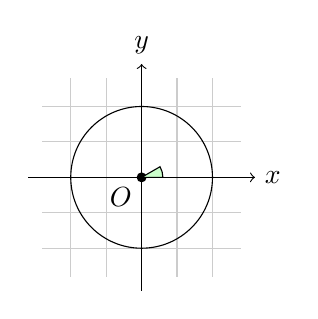
\begin{tikzpicture}[scale=0.9]
    \draw[step=0.5, thin, gray!40] (-1.4,-1.4) grid (1.4,1.4);  % help lines
    \draw[->] (-1.6,0) -- (1.6,0) node[right] {$x$};
    \draw[->] (0,-1.6) -- (0,1.6) node[above] {$y$};
    \draw (0,0) circle [radius=1];
    \fill (0,0) circle (2pt);
    \node[below left] at (0,0) {$O$};
    % filldraw = fill AND stroke; the wedge from 0 to 30 degrees
    \filldraw[fill=green!20, draw=black]
        (0,0) -- (3mm,0) arc [start angle=0, end angle=30, radius=3mm] -- cycle;
\end{tikzpicture}
\end{center}

% The other path primitives, all in one picture:
%   rectangle  ellipse  arc  -- cycle (closes the path)
%   .. controls .. ..  (bezier)     -|  (horizontal then vertical)
%   |-  (vertical then horizontal)
\begin{center}
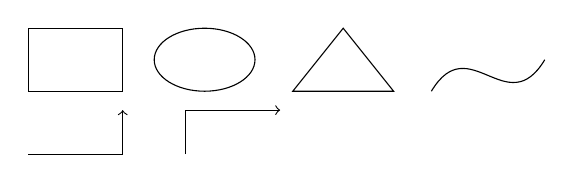
\begin{tikzpicture}[scale=0.8]
    \draw (0,0) rectangle (1.5,1);
    \draw (2.8,0.5) ellipse (0.8 and 0.5);
    \draw (4.2,0) -- (5,1) -- (5.8,0) -- cycle;
    \draw (6.4,0) .. controls (7,1) and (7.6,-0.5) .. (8.2,0.5);
    \draw[->] (0,-1) -| (1.5,-0.3);
    \draw[->] (2.5,-1) |- (4,-0.3);
\end{tikzpicture}
\end{center}

\subsection{Options: colour, thickness, arrows, fill}
% Thickness keywords, thinnest to thickest:
%   ultra thin, very thin, thin, semithick, thick, very thick, ultra thick
% Arrow tips: ->  <-  <->  -stealth
% GOTCHA: -stealth' (with the prime) is from the OLD arrows library. On a
% current TeX Live it errors with "Unknown arrow tip kind" unless you load
% \usetikzlibrary{arrows}, which this file does.
\begin{center}
\begin{tikzpicture}
    \draw[blue, thick] (0,0) circle (0.5);
    \draw[red, very thick, dashed] (1.5,0) -- (3.5,0);
    \draw[->]        (4,0.6)  -- (6,0.6);
    \draw[<->]       (4,0.2)  -- (6,0.2);
    \draw[-stealth, thick]           (4,-0.2) -- (6,-0.2);
    \draw[-stealth', rounded corners] (4,-0.6) -- (5,-0.6) -- (6,-1);
    \fill[red!50] (6.8,0) circle (3pt);
    \draw[fill=blue!10, draw=black, rounded corners] (7.4,-0.4) rectangle (9,0.4);
\end{tikzpicture}
\end{center}

\subsection{Nodes and relative positioning}
% A node is a box with text, a shape and a NAME. \draw then connects nodes by
% name instead of by coordinate.
%
%   \node[options] (name) at (x,y) {text};
%
% GOTCHA: right=of a  (positioning library) leaves a gap between the node
% BORDERS. The old  right of=a  measures CENTRE TO CENTRE and makes wide
% nodes overlap. Always use the = form.
%
% Anchors: above below left right "above left", or (a.north), (a.south east).
% Inside a node, \\ needs align=center or text width=...
\begin{center}
\begin{tikzpicture}[node distance=0.5cm]
    \node[block] (eat)    {Eat};
    \node[block, right=of eat]    (sleep)  {Sleep};
    \node[block, right=of sleep]  (code)   {Code};
    \node[block, right=of code]   (repeat) {Repeat};
    \draw[arrowline] (eat)   -- (sleep);
    \draw[arrowline] (sleep) -- (code);
    \draw[arrowline] (code)  -- (repeat);
    % a mid-path label
    \draw[arrowline] (repeat.south) -- ++(0,-0.7)
          node[right, black] {loop forever};
\end{tikzpicture}
\end{center}

\subsection{\texttt{\textbackslash foreach} loops}
% \foreach \x in {0,...,4}   is a RANGE. {0,2,...,10} counts in twos.
% GOTCHA: arithmetic in a coordinate must be BRACED -- (0,{2-\y}) not (0,2-\y).
% Multiplication like (2*\x, 2*\y) happens to work without braces because the
% coordinate parser handles *, but subtraction does not.
\begin{center}
\begin{tikzpicture}[scale=0.55]
    \foreach \x in {0,...,4}{
        \foreach \y in {0,...,2}{
            \draw[fill=customblue!10] (1.4*\x, 1.4*\y) rectangle ++(1,1);
        }
    }
\end{tikzpicture}
\end{center}

% Generating named nodes in a loop and then wiring them up -- the classic MLP.
\begin{center}
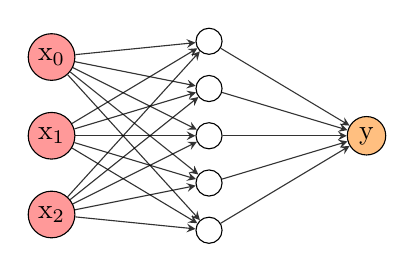
\begin{tikzpicture}[
    inputnode/.style={draw, circle, fill=red!40, inner sep=2pt},
    hiddenunit/.style={draw, circle, minimum size=9pt},
    outnode/.style={draw, circle, fill=orange!50, inner sep=2pt},
    weights/.style={-stealth, thin, opacity=0.8},
]
    \node[inputnode] (x0) at (0, 1)  {$\mathrm{x}_0$};
    \node[inputnode] (x1) at (0, 0)  {$\mathrm{x}_1$};
    \node[inputnode] (x2) at (0,-1)  {$\mathrm{x}_2$};
    \foreach \i in {2,1,0,-1,-2}
        \node[hiddenunit] (h\i) at (2, \i*0.6) {};
    \node[outnode] (y0) at (4,0) {$\mathrm{y}$};

    \foreach \x in {x0, x1, x2}
        \foreach \h in {h2,h1,h0,h-1,h-2}
            \draw[weights] (\x) -- (\h);
    \foreach \h in {h2,h1,h0,h-1,h-2}
        \draw[weights] (\h) -- (y0);
\end{tikzpicture}
\end{center}

\subsection{Styles, scopes and the \texttt{calc} library}
% Styles can be global (\tikzset in the preamble, as with "block" above) or
% local to one picture. They can inherit from each other.
% \begin{scope}[...] applies options to part of a picture only.
% ($(a)!0.5!(b)$) is the midpoint; !0.25! is a quarter of the way.
% \node[fit={(a)(b)}] draws a box around several existing nodes.
\begin{center}
\begin{tikzpicture}[
    module/.style={draw, very thick, rounded corners, minimum width=14ex,
                   align=center},
    embmodule/.style={module, fill=red!20},
    mhamodule/.style={module, fill=orange!20},
    lnmodule/.style={module, fill=yellow!20},
    arrow/.style={-stealth', thick, rounded corners},
    node distance=0.45cm,
]
    \node (inputs) {Inputs};
    \node[above=of inputs, embmodule] (emb) {Input\\Embedding};
    \node[above=of emb, draw, thick, circle] (plus) {$+$};
    \node[above=of plus, mhamodule] (mha) {Multi-Head\\Attention};
    \node[above=of mha, lnmodule] (norm) {Add \& Norm};
    \node[above=of norm] (outputs) {Outputs};

    \draw[arrow] (inputs) -- (emb);
    \draw[arrow] (emb)    -- (plus);
    \draw[arrow] (plus)   -- (mha);
    \draw[arrow] (mha)    -- (norm);
    \draw[arrow] (norm)   -- (outputs);

    % a residual connection: midpoint, then out to the left, then back in
    \coordinate (res) at ($(mha.south)!0.5!(plus.north)$);
    \coordinate[left=of norm] (resleft);
    \draw[arrow] (res) -| (resleft) -- (norm);

    % a box fitted around two nodes, labelled on the left
    \node[fit={(mha)(norm)}, draw, thick, rounded corners,
          label=left:$\mathrm{N}\times$] {};

    \begin{scope}[blue, thick]
        \draw (3,0) -- (3,1);      % these two inherit blue+thick from the scope
        \draw (3,1) -- (4,1);
    \end{scope}
\end{tikzpicture}
\end{center}

% TikZ also works inline, inside a sentence or inside a node:
Inline TikZ: \tikz \draw[scale=0.1, blue] plot[domain=0:6.28] (\x,{sin(\x r)});

% Libraries worth knowing:
%   positioning  right=of, above=of
%   calc         ($(a)!0.5!(b)$)
%   fit          a node fitted around other nodes
%   arrows       the primed tips: stealth' latex' to'
%   arrows.meta  -{Stealth}, -{Latex}
%   shapes.geometric  diamond, trapezium, star
%   intersections     name path / name intersections


% #############################################################################
\section{Two-column layout}
% #############################################################################
% For a whole two-column document (23_A1, 23_C1), put the option on the class:
%       \documentclass[twocolumn]{article}
% and use figure* / table* for anything that must span both columns.
%
% You can also switch mid-document, which is what happens below.
% \twocolumn and \onecolumn both start a new page.
%
% GOTCHA: \newpage in twocolumn mode ends the COLUMN, not the page.
% \clearpage ends the page and flushes floats.
% The alternative, \usepackage{multicol}, makes a two-column REGION rather
% than a two-column document -- but floats do not work inside it, so it is the
% wrong tool for reproducing a paper.

\twocolumn

\subsection{Text in two columns}
This paragraph is set in two-column mode. Everything you have seen so far --
lists, maths, tables, figures -- behaves identically here; the only difference
is that \verb|\linewidth| is now the width of one column rather than the width
of the page, which is exactly why sizing images with \verb|\linewidth| rather
than \verb|\textwidth| is the safer habit.

A normal \texttt{figure} or \texttt{table} float stays inside its column. To
span both columns you need the starred forms, and they can only be placed at
the top of a page.

\begin{table}[H]
    \centering
    \caption{A table inside one column.}
    \label{tab:incolumn}
    \begin{tabular}{|c|c|}
        \hline
        $n$ & $n^2$ \\ \hline
        1 & 1 \\ \hline
        2 & 4 \\ \hline
        3 & 9 \\ \hline
    \end{tabular}
\end{table}

An equation also narrows to the column:
\begin{equation}
    \zeta(s) = \sum_{n=1}^{\infty} \frac{1}{n^s}.
    \label{eq:zeta}
\end{equation}

Equation~\eqref{eq:zeta} converges for $\mathrm{Re}(s) > 1$, and
Table~\ref{tab:incolumn} sits happily inside a single column.

\onecolumn

\section*{Back to one column}
% A starred section: no number, and no entry in the table of contents.
% 22_C2 ends with exactly this -- an unnumbered "Conclusion".
\addcontentsline{toc}{section}{Back to one column}
% ^ put the starred section back into the ToC by hand, if you want it there.

That is every construct from the nine past papers. If you can reproduce this
file from scratch, you can reproduce any of them.

\end{document}
